\chapter{Prehľad problematiky}

V tejto kapitole vysvetlíme, čo je rozšírená realita a ako bola definovaná. Popíšeme na~čo všeobecne slúži a akými spôsobmi sa používa. Popíšeme kedy nastáva oklúzia a definujeme oklúder.

\section{Definícia rozšírenej reality}

Rozšírená realita (po anglicky \emph{augmented reality}, skrátene \emph{AR}) je počítačom rozšírený pohľad na reálny svet. Je to variácia virtuálnej reality, v ktorej používateľ nevníma svet okolo seba a je prenesený do sveta virtuálneho. Tento virtuálny svet je úplne umelý a nezávislý. Oproti tomu, pri rozšírenej realite používateľ naďalej vníma skutočný svet okolo seba doplnený o virtuálne objekty \cite{Azuma97}. Ronald T. Azuma definuje rozšírenú realitu tromi pravidlami \cite{Azuma97}.

\begin{enumerate}
\item Rozšírená realita musí kombinovať reálne a virtuálne objekty.
\item Aplikácia musí prebiehať v reálnom čase a nejakým spôsobom reagovať na zmeny v prostredí, teda byť interaktívna.
\item Rozšírená realita musí byť registrovaná v trojdimenzionálnom priestore. To znamená, že musí korektne registrovať pohľad kamery s virtuálnym svetom a správne identifikovať, na ktoré pozície je potrebné vykresliť (po anglicky \emph{render}) virtuálne objekty.
\end{enumerate}

Cieľom rozšírenej reality môže byť v jednoduchšom prípade prezentovať používateľovi nejaké informácie (napríklad informácie o určitých skutočných objektoch, ako je ich vzdialenosť, poloha, identifikácia a podobne), alebo vykreslovať neskutočné objekty tak, aby vyzerali ako skutočné a patriace do okolitého prostredia. V druhom prípade je potrebné, aby boli tieto objekty trojdimenzionálne a vykresľovali sa správne v súlade s perspektívou a skutočnými objektami (napríklad prekrývali objekty za nimi, ale boli prekryté objektmi pred nimi) \cite{Azuma01}. V prvom prípade je však podľa Azumovej definície stále potrebné, aby sa dané informácie vykreslovali vo výstupe na správne miesta, závisiace od vstupu kamery, alebo iných senzorov. Príklady oboch sú uvedené v nasledujúcej kapitole.

Rozšírená realita sa, rovnako ako virtuálna realita, nemusí nutne týkať iba vizuálneho obrazu. Teoreticky by mohla ovplyvňovať každý druh senzorického vnímania. Je to však obtiažna úloha, pretože na rozdiel od virtuálnej reality, v
ktorej stačí tieto umelé zmyslové podnety len generovať, rozšírená realita musí upravovať skutočný svet. To znamená, že okrem dopĺňania virtuálnych objektov občas potrebuje retušovať skutočné objekty, aby zanikli. Na to, aby sa to dalo dosiahnuť je potrebné vedieť zablokovať určitú časť pôvodného vnemu \cite{Bimber05}.

V prípade zraku je potrebné prekresliť skutočný objekt pozadím, ktoré sa nachádza za ním. Pri sluchu je filtrovanie jednotlivých zvukových stôp zo zmixovaného vstupu a navyše v reálnom čase (napríklad odfiltrovanie hlasu niektorej osoby v miestnosti) obtiažnejším problémom.

Rozšírená realita sa z praktických dôvodov obvykle zameriava na obraz. Týmto aspektom sa zaoberá aj táto práca.

\section{Účel}

Dôvodov pre vývoj rozšírenej reality je niekoľko. Pre používateľa môže byť rozšírená realita jedným z najjednoduchších spôsobov ako získavať určité druhy
informácií. Toto môže zefektívňovať a zjednodušovať jeho skutočnú prácu. Obzvlášť prakticky vyzerajú napríklad koncepty, pri ktorých má používateľ špeciálne okuliare, ktoré mu zobrazujú požadované dáta zo senzorov a databáz priamo na sklá a používateľovi ostávajú voľné ruky na prácu.

Dobrým príkladom je napríklad aplikácia firmy Boeing, vyvinutá pre mechanikov servisujúcich lietadlá. Keď mechanik odstráni niektorý z krycích panelov na lietadle, môže namieriť kameru tabletu na zväzky káblov a rozvodov, ktoré sa pod ním nachádzajú. Softvér v reálnom čase na obrazovku dopĺňa údaje o tom, ktorý kábel, alebo trubica kam vedie a na čo slúži. Šetrí sa tak množstvo času oproti vyhľadávaniu v~hrubých manuáloch.

Rozšírená realita má samozrejme taktiež široké spektrum využitia v~zábave alebo marketingu.

\section{Zariadenia}

Rozšírená realita môže byť prezentovaná používateľovi buď priamo (napríklad vykreslovaním na priehľadný displej, cez ktorý je priamo vidno okolité prostredie), alebo nepriamo, čiže vykreslovaním do záznamu z videokamery, ktorý je vzápätí po rozšírení prezentovaný používateľovi na nepriehľadný displej.

\begin{figure}[h]
 \centering
 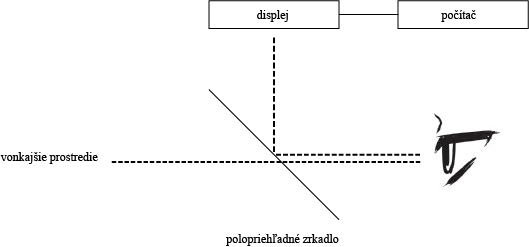
\includegraphics[scale=0.6]{pictures/schema-hmd}
 \caption{Schéma priamej rozšírenej reality}
 \label{prama-realita}
 \end{figure}

V prípade priamej optickej rozšírenej reality za použitia priehľadného displeja sa obvykle používa nejaký typ okuliarov, alebo helmy. Tieto okuliare obsahujú šikmú poloreflexnú plochu, cez ktorú je priamo vidno, ale taktiež odráža obraz z malého displeja umiestneného nad ňou, alebo pod ňou \cite{Bimber05}. Keď sa cez ne používateľ pozrie, obrazy sa mu skombinujú (znázornené na obrázku \ref{prama-realita}).

\begin{figure}[h]
 \centering
 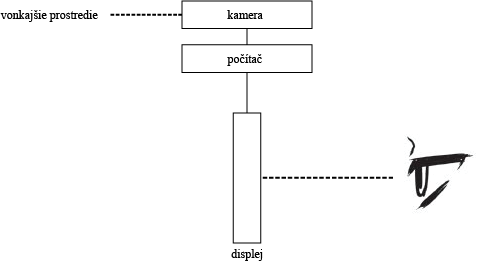
\includegraphics[scale=0.6]{pictures/schema-hmd-2}
 \caption{Schéma sprostredkovanej rozšírenej reality}
 \label{nepriama-realita}
 \end{figure}

Pre videom sprostredkovanú rozšírenú realitu sa používajú ľubovoľné zariadenia s~obrazovkami, ako sú telefóny, tablety, či počítače. Ani v tomto prípade však nie je vylúčené použitie špeciálnej helmy. Takéto helmy sa označujú ako HMD z anglického \emph{head-mounted display}. Podľa vysvetleného použitia sa delia na \emph{optical see through} (priame) a \emph{video see through} (sprostredkované). V demo aplikácií, ktorá bola vyvinutá ako súčasť tejto práce, ukazujeme sprostredkovanú rozšírenú realitu pomocou počítača, ku ktorému je pripojená kamera (znázornené na obrázku \ref{nepriama-realita}).

\section{Definícia oklúzie}

Oklúzia (po anglicky \emph{occlusion culling}), je proces počas ktorého algoritmus rozhoduje, ktoré objekty alebo prípadne časti objektov sú na scéne viditeľné. Pokiaľ je nejaký objekt sčasti alebo kompletne skrytý za iným objektom, znamená to, že je okludovaný a teda sčasti alebo vôbec nie je viditeľný (ilustruje obrázok \ref{sonofman}). Objekt, ktorý ho zakrýva sa nazýva oklúderom (po anglicky \emph{occluder}).

Oklúzia sa obvykle používa ako optimalizačná metóda (nie je potrebné vykresľovať pixely, ktoré budú napokon prekryté), v rozšírenej realite sa dá využiť tak, aby ilúzia pôsobila reálnejšie.

\begin{figure}[h]
 \centering
 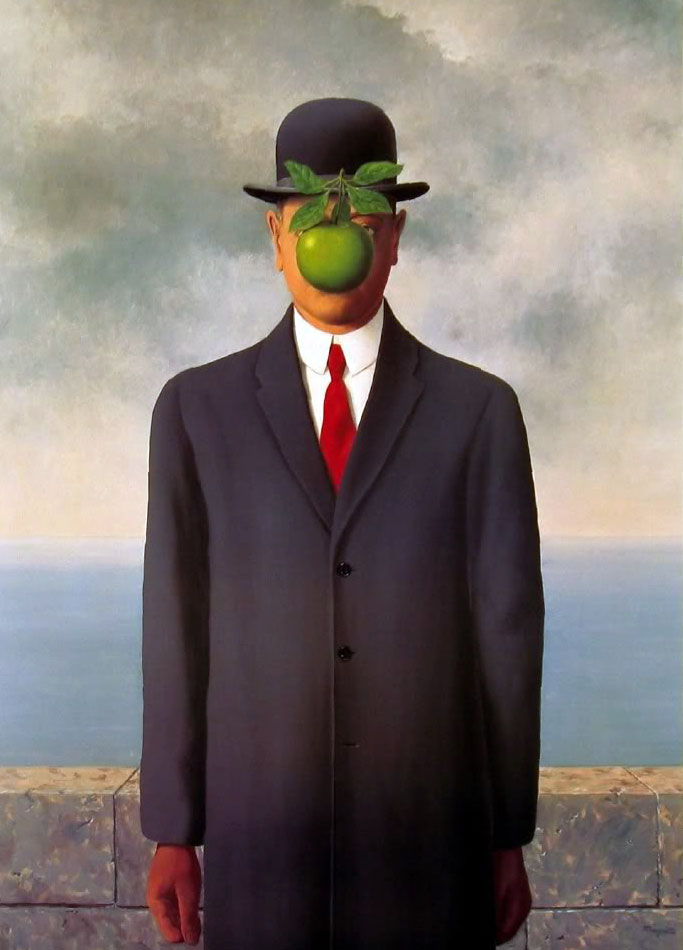
\includegraphics[scale=0.3]{pictures/sonofman.jpg}
 \caption[Na maľbe je mužova tvár čiastočne zakrytá jablkom. V 3D priestore by bolo jablko oklúderom.]{Na maľbe je mužova tvár čiastočne zakrytá jablkom\footnotemark. V 3D priestore by bolo jablko oklúderom.}
 \label{sonofman}
\end{figure}
\footnotetext{Obraz \emph{The Son of Man} namaľoval belgický umelec René Magritte.}